\section{Introduction}

\begin{frame}{Introduction}
    In this presentation, we will be discussing quantum channels and how they developed from classical channels. But before that, we need to define what quantum channels
    are and what they operate on.
    Quantum channels operate on Density Matrices, which are mathematical constructs that hold all information about a quantum state. They can be defined as:
    \begin{equation}
        \rho = \sum_{i}p_i | \psi_i \rangle \langle \psi_i |   
    \end{equation}
    where $\psi_i$ is the $i^th$ state occuring with probability $p_i$
\end{frame}

\begin{frame}{Introduction}
    A quantum channel acts as a linear \textit{Completely Positive Trace Preserving (CPTP)} map from one density matrix to the other. This means that the product state
    of the system and the environment stays positive throughout the transformation, and the trace remains constant. These two properties are essential for a channel to
    be physically viable and make sense in the real world.\\
    It is usually denoted with $\mathcal{N}$ and the state generated after the application of the channel is $\mathcal{N} (\rho)$.\\
    Generally, this channel is second one of the three steps that happen in the process of sending information from A to B, the others being encoding and decoding.
    These three steps have been illustrated in the following figures.
\end{frame}

\begin{frame}
    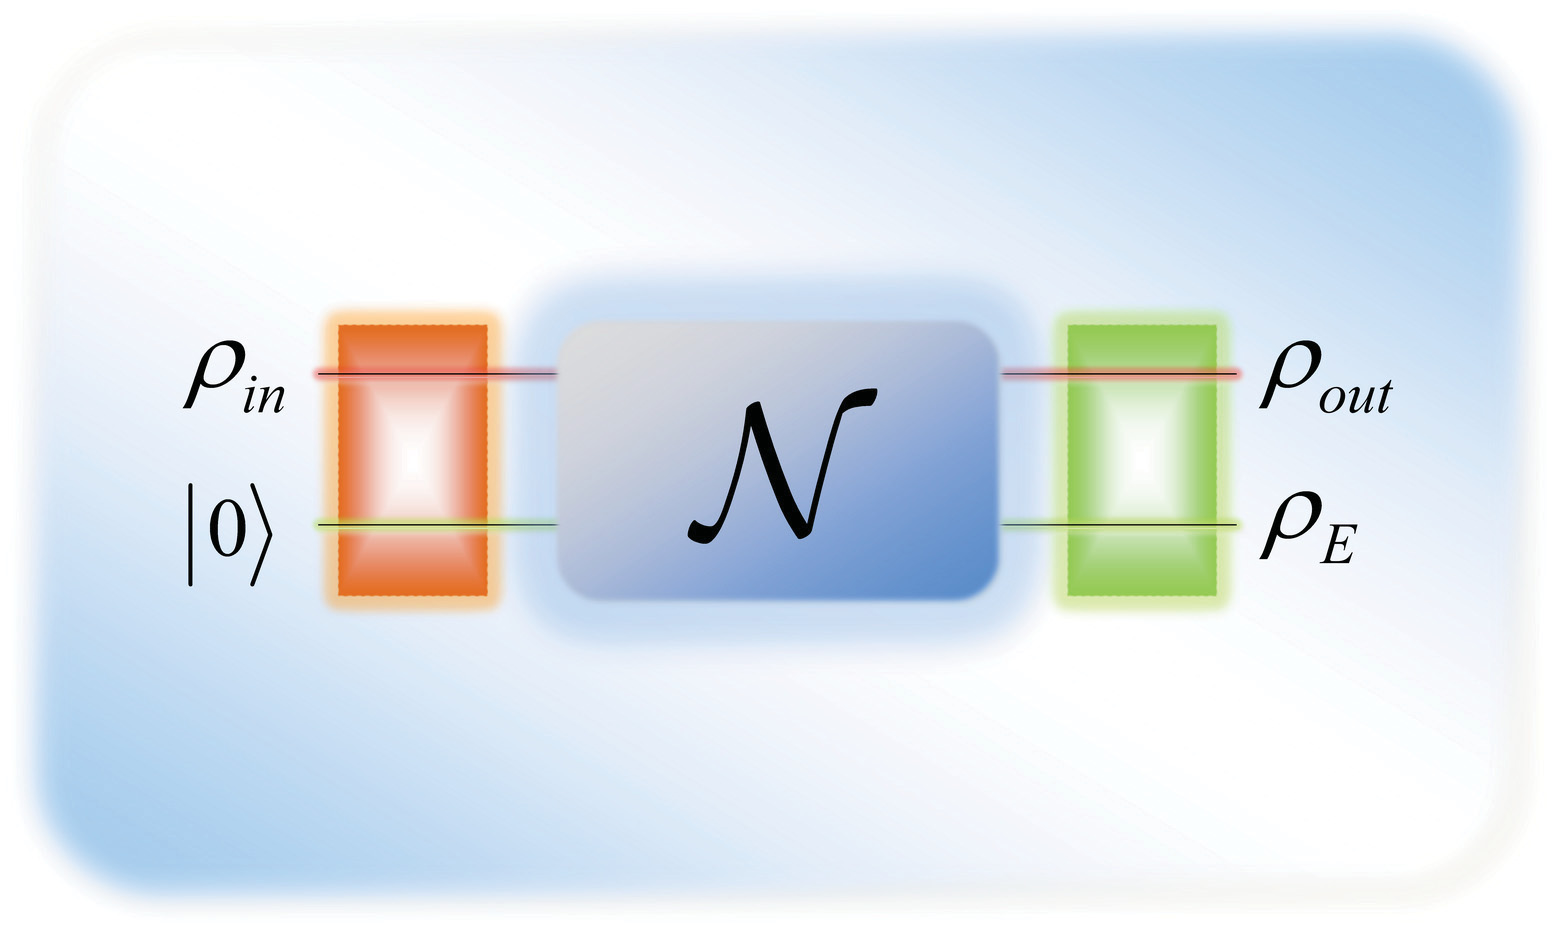
\includegraphics[scale=0.1]{channel2.png}
    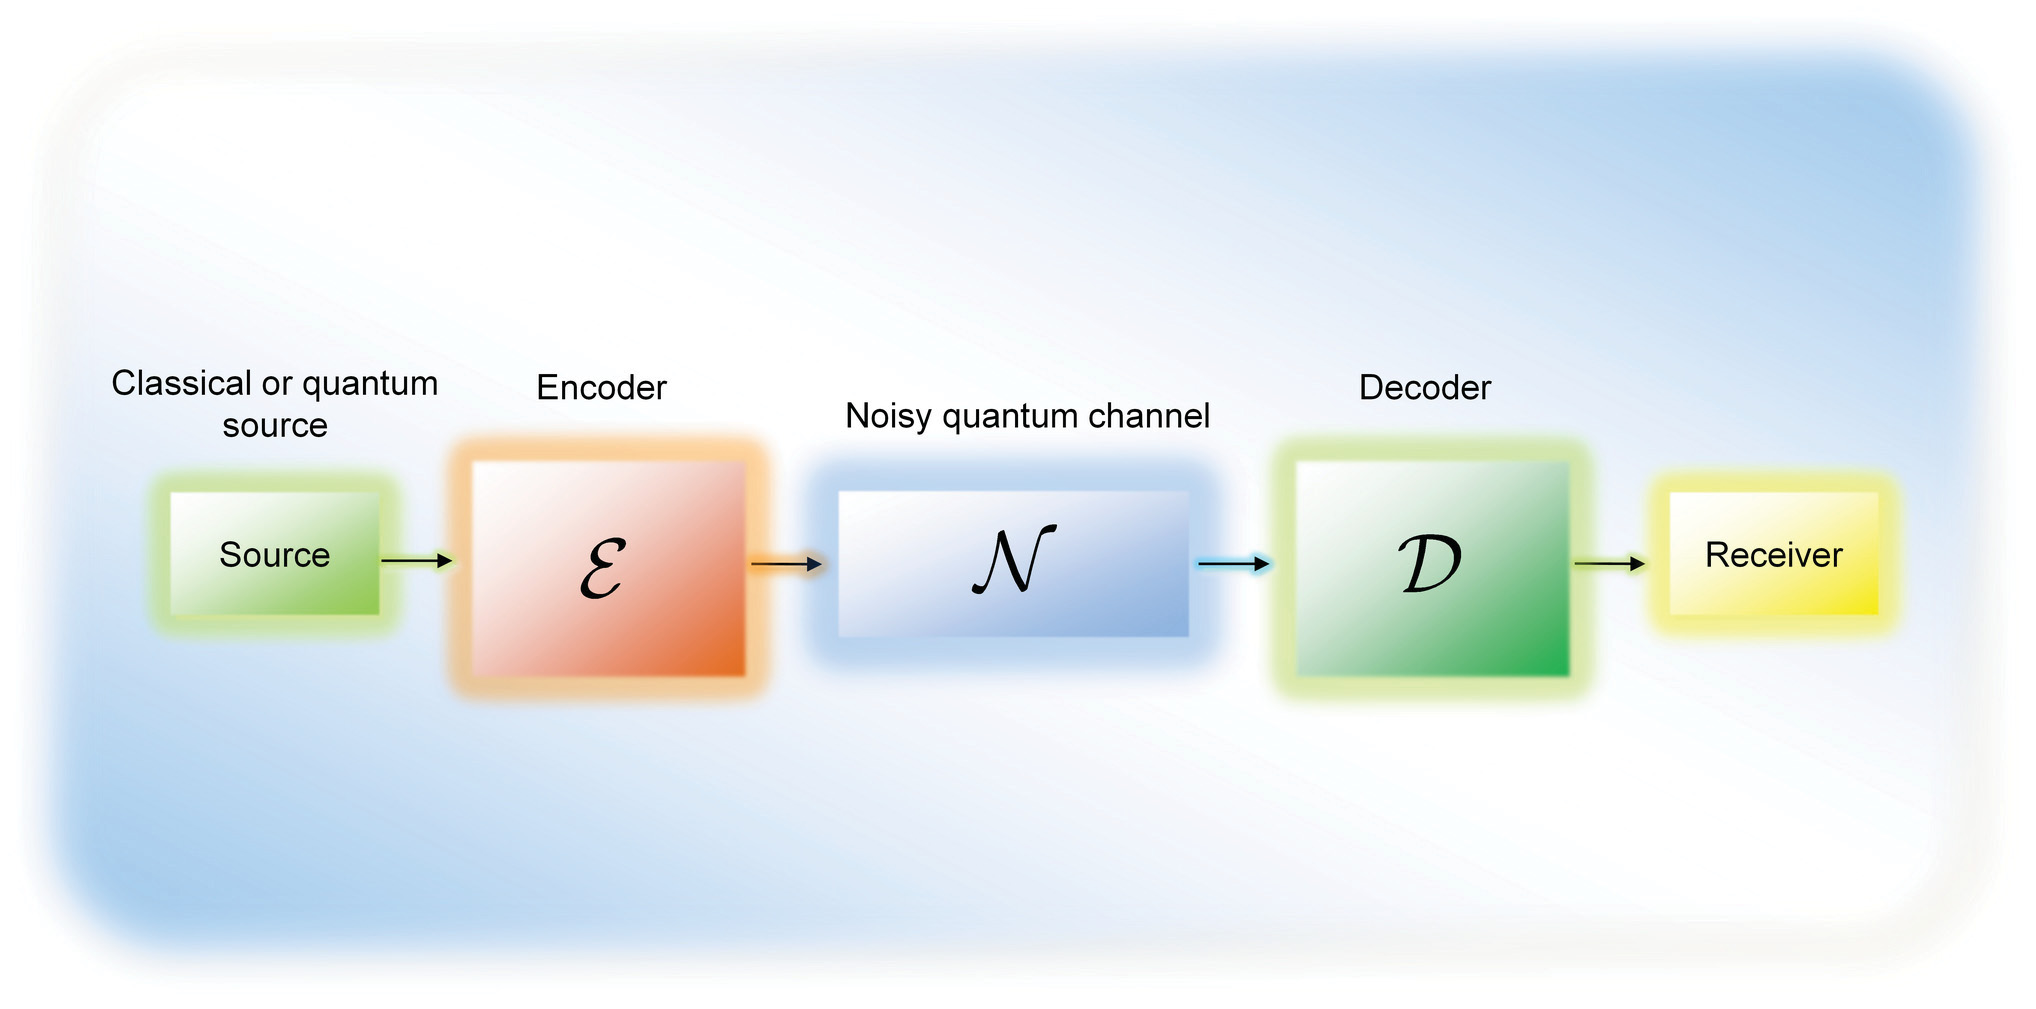
\includegraphics[scale=0.15]{channel1.png}
\end{frame}

\begin{frame}{Kraus Representation}
    Quantum channels are often represented in what is called the Kraus form (or the Choi-Kraus representation). In this form, quantum channels can be defined
    as linear combination in the following way:
    \begin{equation}
        \mathcal{N}(\rho) = \sum_i K_i \rho K_i^\dagger 
    \end{equation}
    where $\sum_i K_i^\dagger K_i = \mathbb{I} $\\
    The Kraus representation is very useful in as a tool for analysing quantum channels, and makes several problens easier to solve. Kraus operators and their
    uses show up at many useful places throughout Quantum information theory. It makes channels easier to understand as well, by decomposing them into several
    "sub-channels".
\end{frame}

\begin{frame}{Von Neumann Entropy}
    
\end{frame}

\begin{frame}{Quantum Relative Entropy}
    
\end{frame}

\begin{frame}{Quantum Mutual Information}
    
\end{frame}